\documentclass[12pt]{article}
\usepackage{url}
\usepackage{graphicx}
\usepackage{float}
\usepackage{amsmath}
\usepackage{amsfonts}
\usepackage{amssymb}
\setlength{\parindent}{0mm}
\title{\bf CCP5 Funding Application for the Fortran Modernisation Workshop}
\author{Fatima Chami\footnote{fatima.chami@stfc.ac.uk},
  Wadud Miah\footnote{wadud.miah@nag.co.uk},
  Filippo Spiga\footnote{fs395@cam.ac.uk} and
  Kyle Fernandes\footnote{kj333@cam.ac.uk}}
\date{\today}

\begin{document}
\maketitle

%
\section{Introduction}
The Fortran Modernisation Workshop\footnote{\url{http://www.nag.co.uk/content/fortran-modernization-workshop}} is a two day event
that was designed to
address the software engineering needs specifically for the computational science community using the Fortran programming language.
It covers the more modern features of Fortran, namely 90, 95, 2003 and 2008, to encourage attendees to modernise their legacy
Fortran 77 and 66 codes. It also aims to teach attendees how to write portable, efficient, extensible and modular code in Fortran for
multi-scale and multi-physics computational science. The workshop is run by a number of organisers which are listed in the author's
list who are computational scientists with extensive coding experience, making them qualified to run this workshop. In addition, the
Digital Technology Group~\footnote{\url{http://www.cl.cam.ac.uk/research/dtg/naps/}} from Cambridge University also attend to
present their CamFort Fortran verfication tool and Allinea~\footnote{\url{www.allinea.com}} also present their debugging and
profiling tools for Fortran. Although there are a number of Fortran and software engineering workshops run by the Archer HPC
service and the Software Sustainability Institute, such workshops tend to be very generic and do not address any particular
academic community which makes Fortran Modernisation Workshop workshop very unique. \\

The topics that are covered in this workshop are listed below:
\begin{itemize}
\item Software engineering for computational science;
\item Modern Fortran standards;
\item NetCDF and HDF5 scientific file formats for data sharing in Fortran;
\item GNU Automake to automate the build process;
\item pFUnit unit testing framework for testing Fortran codes;
\item Fortran verification using CamFort;
\item Doxygen for Fortran code documentation;
\item Git version control for collaborative code development;
\item In-memory visualisation using PLplot in Fortran;
\item IEEE Floating Point Exception Handling
\item Fortran interoperability with C, Python and R;
\item Introduction to parallelism for Fortran;
\item Debugging and profiling Fortran using Allinea DDT and MAP.
\end{itemize}
The technologies listed above cover the code development lifecycle as well as the computational science workflow,
again making this workshop very unique and specific to computational science. Further info can be found at:
\url{http://www.fortran.bcs.org/2016/bcs_fmw_miahw.pdf}
During the workshop registration, the attendees
were asked which versions of the Fortran standard they were using, and this is shown in Figure~\ref{fortran_usage:png}. 
\begin{figure}[H]
\begin{center}
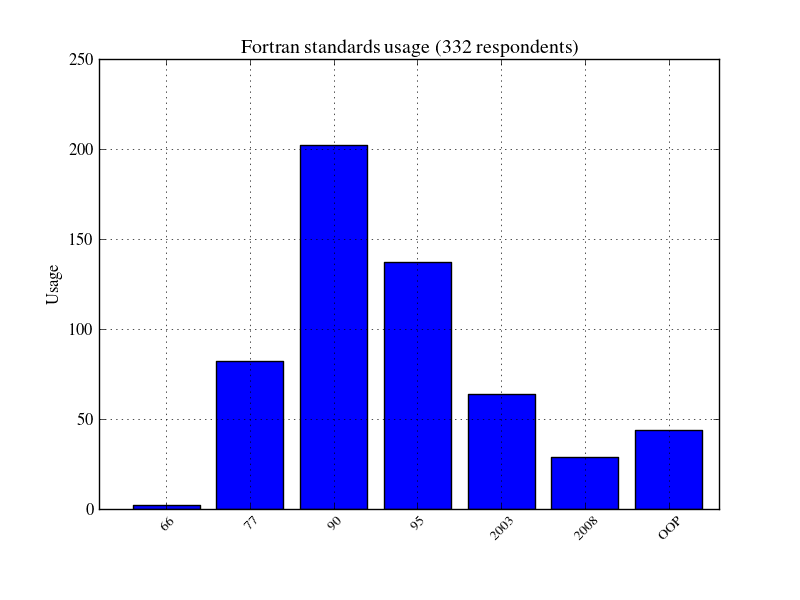
\includegraphics[width=13cm,height=9cm]{fortran_usage.png}
\caption{Fortran standards usage}\label{fortran_usage:png}
\end{center}
\end{figure}
Figure~\ref{fortran_usage:png} shows that the most widely used standard is Fortran 90, but there still exists a number of
Fortran 77 users. In addition, adoption of the newer standards such as 2003 and 2008 is still lacking which needs wider
adoption that aids better software engineering. Thus, ones of the aims of the workshop is to address this shortfall. \\

The workshop feedback form listed the technologies that attendees intend to use which is shown in Figure~\ref{future:png}
which shows that attendees intend to use the modern features of Fortran.
\begin{figure}[H]
\begin{center}
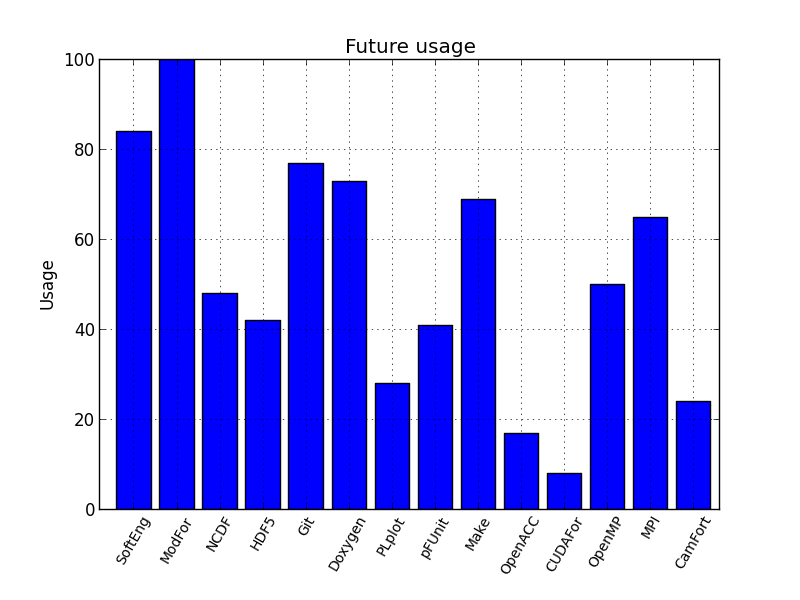
\includegraphics[width=13cm,height=9cm]{future.png}
\caption{Future technology usage by attendees}\label{future:png}
\end{center}
\end{figure}
What Figure~\ref{future:png} also shows that there is a lack of interest in Fortran verfication techniques such as
pFUnit and CamFort. This is a trend the workshop organisers have noticed and intend to emphasise the importance
of code verfication which is generally not very well covered for the Fortran programming language. 
\section{History of the Workshop}
The Fortran Modernisation Workshop has been hosted at a number of sites which is listed in Table~\ref{fmw:sites} which shows
an average of 33.5 attendees. 
\begin{table}[H]
\centering 
\begin{tabular}{|c|c|c|c|}
\hline
{\bf Site} & {\bf Date} & {\bf No. attendees} & {\bf Rating} \\ \hline
Cambridge University & March 2016 & 44 & 4.058/5 \\ \hline
Oxford University & July 2016 & 31 & 3.52/5 \\ \hline 
University of Southampton & July 2016 & 44 & 4.286/5 \\ \hline
CCFE & August 2016 & 11 & 3.445/5 \\ \hline
Queen Mary London & September 2016 & 41 & 4.143/5 \\ \hline
STFC Daresbury & October 2016 & 30 & 4.556/5 \\ \hline
\end{tabular}
\caption{Fortran Modernisation Workshop sessions}
\label{fmw:sites}
\end{table}
The current list of future workshop sessions are shown in Table~\ref{fmw:future} and the workshop organisers are in
discussion with other sites regarding hosting the workshop. 
\begin{table}[H]
\centering 
\begin{tabular}{|c|c|c|}
\hline
{\bf Site} & {\bf Date} & {\bf Number of registrations} \\ \hline
Manchester University & February 2017 & 20 \\ \hline
University of Reading & February 2017 & 25 \\ \hline 
\end{tabular}
\caption{Future Fortran Modernisation Workshop sessions}
\label{fmw:future}
\end{table}
The registrations for the workshops listed in Table~\ref{fmw:future} are still open and are increasing. 
\section{Summary}
As can be seen from Table~\ref{fmw:sites} the workshop has been hosted at six sites and received very positive ratings.
Future sessions are listed in Table~\ref{fmw:future} and the workshop is continuously being improved from the feedback received.
The workshop was attended mainly by academics as well as attendees from industry, particularly at the STFC Daresbury session. \\


%\bibliographystyle{abbrv}
%\bibliography{fortran_usage}

\end{document}

